\documentclass[10pt]{article}
\usepackage{icmlko}

\icmlmeta{IP 파운데이션 월드모델}{70}{반쯤 아는 방향은 모르느니만 못했다}{노트 69의 뒤집기를 정당한 절차로 바꾸니 라벨 넷으로는 손해였고 서른둘부터 값을 했다}

\begin{document}

\twocolumn[
\icmlheader

\begin{abstract}
노트 69는 애니메이션의 축 방향을 \textbf{답을 보고} 뒤집었다 --- 진단이지
채택이 아니었다. 정당한 절차로 바꿨다. \textbf{대상 라벨 $k$건만 보고 방향을
정한 뒤 나머지로 평가한다.} 보정에 쓴 $k$건은 평가에서 빼고, 라벨 탈추세도
$k$건 안에서만 한다(전표본 추세 계수를 쓰면 나머지 $n-k$건이 새어 든다 ---
노트 35 · 54 · 64와 같은 종류라 \texttt{factor\_space}에 탈추세 전 라벨을
내보내게 고쳤다). 세 방식을 쟀다. \textbf{놀랍게도 사후 부호가 구조 교정을
이긴다} --- 셀별 $+$0.2945, 도메인별 $+$0.2363, 원 축을 실제로 뒤집는 축 정향
$+$0.2250($k{=}40$). 오정향이 도메인의 성질이 아니라 \emph{쌍}의 성질이기
때문이다. 그리고 정작 중요한 결과는 작은 $k$에 있다. \textbf{$k{=}4$에서
보정은 손해다} --- 짝지은 차이 $-$0.0583, $k{=}8$에서 $-$0.0206. 방향을 반쯤
알면 모르느니만 못하다. 틀린 뒤집기가 안 뒤집기보다 두 배 나쁘기 때문이다.
구간이 0을 넘는 것은 \textbf{$k{=}32$부터}이며($+$0.1093 {[}$+$0.021,
$+$0.149{]}), 이것이 노트 69의 ``35건 92\%''를 대체하는 정본 수치다. 마지막으로
값을 치른 뒤에도 일곱 도메인 $+$0.2945는 여섯 도메인 $+$0.3474에 못 미친다 ---
\textbf{여섯 도메인 평균은 방향이 같은 것들만 모여 있어서 낙관적이었다.}
\end{abstract}
]

\section{절차를 정당하게 만든다}

노트 69의 뒤집기는 42셀 평균을 보고 골랐다. 이 프로젝트가 노트 28 · 34 · 35에서
세 번 금지한 것이다. 규약을 바꾼다.

\begin{quote}\fontsize{9.5}{11.5}\selectfont
대상 도메인의 라벨 \textbf{$k$건만} 본다 $\to$ 그 $k$건으로 방향을 정한다 $\to$
\textbf{나머지로 평가한다}. 복제마다 평가 집합을 먼저 고정하고($k_{\max}$를
뺀 크기) 보정 $k$건은 나머지에서 뽑으므로 $k$끼리 비교된다.
\end{quote}

\paragraph{누수를 하나 더 찾았다}
처음 짤 때 보정 상관을 \emph{전표본으로 탈추세한} 라벨의 $k$건으로 쟀다. 추세
계수가 전표본에서 왔으므로 나머지 $n-k$건이 새어 든다. 노트 35(도서 판형) ·
54(붓스트랩 순서) · 64(진단 코드)와 같은 종류다. \texttt{factor\_space}가 탈추세
전 라벨과 시간을 함께 내보내게 고치고, 보정은 $k$건 안에서만 탈추세한다.

\section{세 방식}

\begin{figure*}[t]
\centering
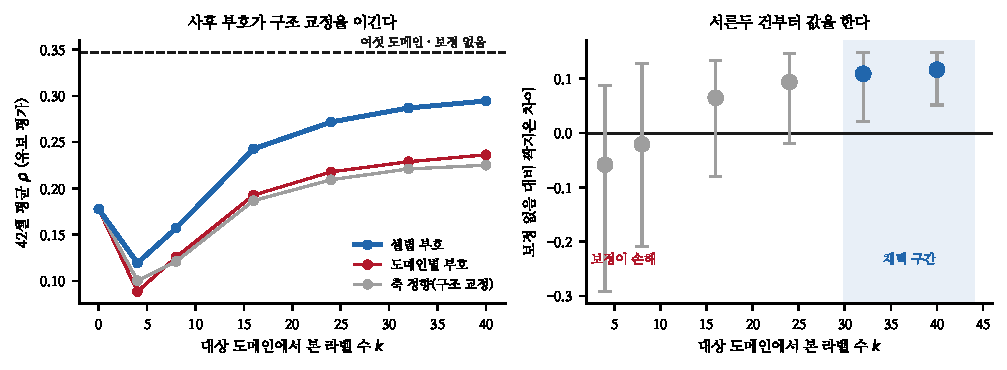
\includegraphics[width=\textwidth]{figs/halfknown.pdf}
\caption{왼쪽 --- $k$와 42셀 평균. 오른쪽 --- 보정 없음 대비 짝지은 차이.}
\end{figure*}

\begin{table}[t]
\centering\tsize
\caption{유보 평가 42셀 평균 $\rho$. 복제 150회.}
\begin{tabular}{lrrr}
\toprule
$k$ & 셀별 부호 & 도메인별 & 축 정향 \\
\midrule
0 & $+$0.1776 & $+$0.1776 & $+$0.1776 \\
4 & $+$0.1193 & $+$0.0884 & $+$0.1001 \\
8 & $+$0.1570 & $+$0.1257 & $+$0.1210 \\
16 & $+$0.2427 & $+$0.1927 & $+$0.1867 \\
32 & $+$0.2869 & $+$0.2288 & $+$0.2210 \\
\textbf{40} & \textbf{$+$0.2945} & $+$0.2363 & $+$0.2250 \\
\bottomrule
\end{tabular}
\end{table}

\textbf{사후 부호가 구조 교정을 이긴다.} 축 정향은 노트 69가 규명한 결함을
직접 고치는데도 진다.

\claimx{오정향은 도메인의 성질이 아니라 \emph{쌍}의 성질이다. 출처와 대상 중
어느 한쪽만 뒤집혀도 그 셀이 뒤집히므로 두 방향의 배타적 논리합이며, 대상
도메인 하나에 부호 하나를 매기는 방식으로는 표현할 수 없다.}{축 정향이 작은
$k$에서 결정을 셋 내리는데(공통 축이 셋) 사후 부호는 하나만 내린다. 결정 수의
차이일 수도 있고 쌍/도메인 구분 때문이 아닐 수도 있다.}

성분 부호는 손댈 필요가 없다는 것도 확인했다. 인자 공간 성분에
$\mathrm{diag}(\pm1)$을 걸면 프로크루스테스 회전이 $R\!\to\!RD$로 흡수하고 릿지가
직교변환에 등변이라 예측이 그대로다. \textbf{뒤집어야 하는 것은 성분이 아니라
축이다.}

\section{반쯤 아는 방향은 손해다}

\begin{table}[t]
\centering\tsize
\caption{보정 없음 대비 짝지은 차이. 같은 복제끼리 뺀다(노트 44).}
\begin{tabular}{lrl}
\toprule
$k$ & $\Delta$ & 95\% 구간 \\
\midrule
4 & \textbf{$-$0.0583} & $[-0.292,\ +0.088]$ \\
8 & $-$0.0206 & $[-0.209,\ +0.129]$ \\
16 & $+$0.0651 & $[-0.079,\ +0.134]$ \\
24 & $+$0.0941 & $[-0.019,\ +0.147]$ \\
\textbf{32} & \textbf{$+$0.1093} & $\mathbf{[+0.021,\ +0.149]}$ \\
40 & $+$0.1169 & $[+0.052,\ +0.149]$ \\
\bottomrule
\end{tabular}
\end{table}

$k{=}4$에서 보정이 \emph{손해}다. 이유가 산술적이다 --- 안 뒤집으면 원래 값을
유지하고 틀리게 뒤집으면 부호가 반대가 되므로, 틀린 뒤집기의 벌은 안 뒤집기의
두 배다. 정확도가 3분의 2쯤이면 기댓값이 음수가 된다.

\claimx{새 카테고리에 방향 보정을 붙이려면 대상 라벨 \textbf{32건}이 필요하다.
그 아래에서는 방향을 추측하지 말고 그대로 쓰는 편이 낫다.}{애니 하나로 정한
문턱이다. 다른 도메인에서는 다를 것이고, 특히 전이 신호가 센 팝업 · 아이돌은
더 적게 들 것이다.}

노트 69는 \emph{부호 판정 정확도}로 ``35건에 92\%''라고 적었다. 그 92\%가
곧바로 이득이 아니다 --- 8\%의 오판이 두 배로 벌을 받으므로 끝단 효과는
훨씬 늦게 양수가 된다. \textbf{정본 수치는 32건이다.}

\section{값을 치르고도 여섯이 낫다}

\begin{table}[t]
\centering\tsize
\caption{같은 유보 규약으로 잰 것들.}
\begin{tabular}{lrl}
\toprule
& 평균 $\rho$ & 95\% 구간 \\
\midrule
\textbf{여섯 도메인 · 보정 없음} & \textbf{$+$0.3474} & $[+0.347, +0.348]$ \\
일곱 도메인 · 보정 없음 & $+$0.1776 & --- \\
일곱 도메인 · 셀별 $k{=}40$ & $+$0.2945 & $[+0.221, +0.354]$ \\
\bottomrule
\end{tabular}
\end{table}

보정은 손실의 88\%를 되찾는다($+$0.1776 $\to$ $+$0.2945, 오라클이 $+$0.3175).
그런데 여섯 도메인에는 여전히 못 미친다. 다른 서른 셀은 애니를 넣어도 안
변하므로, 애니의 열두 셀만 $-$0.24에서 $+$0.18로 올라온 것이다.

\begin{quote}\fontsize{9.5}{11.5}\selectfont
\textbf{그렇다면 여섯 도메인 $+$0.3480은 낙관적이었다.} 그 여섯은 축 방향이
전부 같은 쪽을 가리키는 것들이었고, 그것은 설계가 아니라 우연이다. 새 카테고리
하나를 밖에서 데려오자 그 우연이 깨졌다. \textbf{$+$0.2945가 ``처음 보는
카테고리에 붙였을 때''의 더 정직한 숫자다.}
\end{quote}

\section{한계}

\begin{itemize}[leftmargin=1.1em,itemsep=0.15em]
\item 문턱 32건을 애니 하나로 정했다. 도메인마다 다를 것이 거의 확실하다.
\item $k_{\max}{=}40$이라 평가 집합이 작은 도메인(아이돌 62건 $\to$ 22건)에서
      유보 평가가 몹시 흔들린다. 큰 $k$는 못 본다.
\item 축 정향이 진 이유를 쌍/도메인 구분으로 설명했는데, 결정 수(3 대 1)의
      차이일 수도 있다. 갈라 보지 않았다.
\item 보정을 \emph{채택}은 했으나 정본 파이프라인에 아직 안 넣었다. 파이프라인의
      평가 규약(전표본)과 보정 규약(유보)이 달라 함께 놓는 방식을 정해야 한다.
\item 유보 평가 자체가 전표본 평가보다 낮게 나온다. 여섯 도메인이 $+$0.3474로
      전표본 $+$0.3480과 거의 같은 것은 표본이 커서이고, 작은 도메인에서는
      다를 수 있다.
\end{itemize}

\section{다음}

\begin{enumerate}[leftmargin=1.3em,itemsep=0.15em]
\item 방향 보정을 정본 파이프라인에 넣는다 --- 평가 규약을 유보로 통일할지
      결정한다.
\item 문턱 32건을 다른 도메인에서 다시 잰다. 애니를 빼고 웹툰을 ``새 카테고리''로
      가정하면 얼마인가.
\item 축 정향이 진 이유를 가른다 --- 공통 축 하나만 뒤집게 제한하면 사후 부호를
      따라잡는가.
\item 여덟째 도메인 --- 방향이 또 뒤집힌 것이 오는지 본다. 두 번째 사례가
      나오면 ``우연''이 아니라 ``절반''이다.
\end{enumerate}

\vspace{0.6em}
\hrule height 0.3pt
\vspace{0.5em}
{\footnotesize
\textbf{참고문헌}\\[0.3em]
Wang, Z. et al. (2019). Characterizing and avoiding negative transfer.
\emph{CVPR}, 11293--11302.\\[0.15em]
Rosenstein, M. T. et al. (2005). To transfer or not to transfer.
\emph{NIPS Workshop on Inductive Transfer}.\\[0.15em]
Kaufman, S., Rosset, S., Perlich, C. (2012). Leakage in data mining.
\emph{ACM TKDD}, 6(4), 1--21.\\[0.15em]
Efron, B., Tibshirani, R. J. (1993). \emph{An Introduction to the Bootstrap}.
Chapman \& Hall.\\[0.15em]
Ben-David, S. et al. (2010). A theory of learning from different domains.
\emph{Machine Learning}, 79(1--2), 151--175.
}

\end{document}
